\subsection{OTFS-IM Receiver and Block-Wise MAP Detection}

The OTFS-IM receiver differs from the baseline OTFS receiver because it must recover both the active-position pattern and the QAM symbols placed on the active positions. Therefore, a hard symbol-by-symbol decision is not sufficient. In this thesis, the MP detector is used as a probability engine, and an additional block-wise MAP decision stage is applied to recover the index bits and symbol bits of each IM block.

\subsubsection{Overview of the OTFS-IM Receiver Processing Chain}

After transmission through the delay-Doppler channel, the received time-domain signal is demodulated by the same OTFS demodulation block used in Chapter 3. The output is a delay-Doppler-domain observation denoted by \(\mathbf{Y}_{\mathrm{DD}}\). Since the OTFS-IM transmitter scales active symbols by \(\alpha\), the receiver first normalizes the demodulated grid and the corresponding noise variance:
\begin{equation}
    \mathbf{Y}_{\mathrm{norm}}
    =
    \frac{\mathbf{Y}_{\mathrm{DD}}}{\alpha},
    \qquad
    \sigma^2_{\mathrm{norm}}
    =
    \frac{\sigma^2_{\mathrm{IM}}}{\alpha^2}.
    \label{eq:otfs_im_receiver_normalization}
\end{equation}
The normalized delay-Doppler grid is then passed to the MP detector. The detector estimates, for each delay-Doppler position, the probability that the transmitted value belongs to one of the QAM constellation points or to the inactive value zero. These probabilities are then used by the block-wise MAP stage to decide the most likely activation pattern and active QAM symbols.

Figure~\ref{fig:otfs_im_receiver_flow} summarizes the implemented OTFS-IM receiver flow.

\begin{figure}[H]
    \centering
    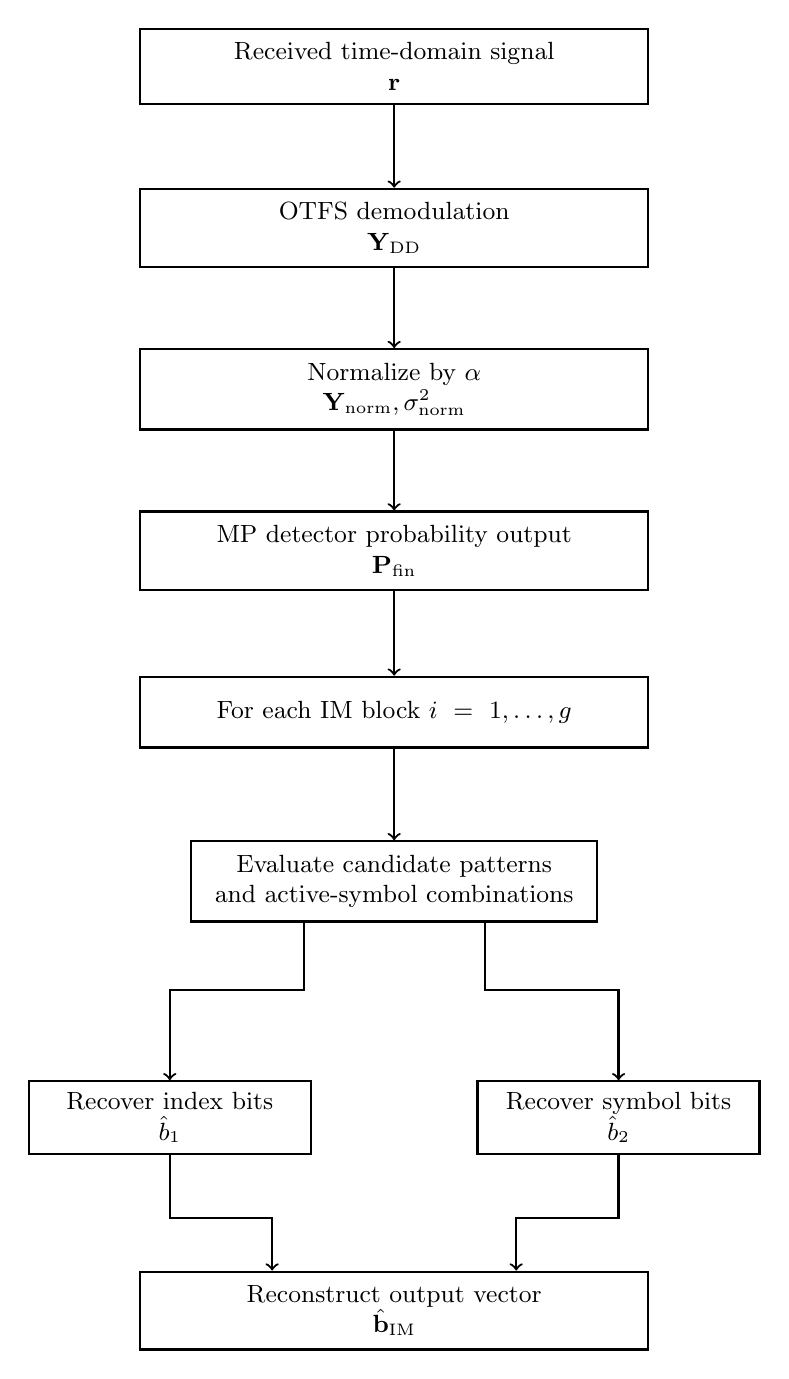
\begin{tikzpicture}[
        block/.style={
            rectangle,
            draw,
            thick,
            align=center,
            text width=6.1cm,
            minimum height=0.9cm,
            font=\small,
            inner sep=5pt
        },
        smallblock/.style={
            rectangle,
            draw,
            thick,
            align=center,
            text width=3.3cm,
            minimum height=0.85cm,
            font=\small,
            inner sep=4pt
        },
        scoreblock/.style={
            rectangle,
            draw,
            thick,
            align=center,
            text width=4.8cm,
            minimum height=0.9cm,
            font=\small,
            inner sep=5pt
        },
        arrow/.style={->, thick}
    ]

        \node[block] (rx) at (0,0) {Received time-domain signal\\\(\mathbf{r}\)};
        \node[block] (demod) at (0,-2.05) {OTFS demodulation\\\(\mathbf{Y}_{\mathrm{DD}}\)};
        \node[block] (norm) at (0,-4.10) {Normalize by \(\alpha\)\\\(\mathbf{Y}_{\mathrm{norm}}, \sigma^2_{\mathrm{norm}}\)};
        \node[block] (mp) at (0,-6.15) {MP detector probability output\\\(\mathbf{P}_{\mathrm{fin}}\)};
        \node[block] (loop) at (0,-8.20) {For each IM block \(i=1,\ldots,g\)};
        \node[scoreblock] (score) at (0,-10.35) {Evaluate candidate patterns\\and active-symbol combinations};
        \node[smallblock] (idx) at (-2.85,-13.35) {Recover index bits\\\(\hat{b}_1\)};
        \node[smallblock] (sym) at (2.85,-13.35) {Recover symbol bits\\\(\hat{b}_2\)};
        \node[block] (bits) at (0,-15.80) {Reconstruct output vector\\\(\hat{\mathbf{b}}_{\mathrm{IM}}\)};

        \draw[arrow] (rx.south) -- (demod.north);
        \draw[arrow] (demod.south) -- (norm.north);
        \draw[arrow] (norm.south) -- (mp.north);
        \draw[arrow] (mp.south) -- (loop.north);
        \draw[arrow] (loop.south) -- (score.north);
        \draw[arrow] ([xshift=-1.15cm]score.south) -- ++(0,-0.85) -| (idx.north);
        \draw[arrow] ([xshift=1.15cm]score.south) -- ++(0,-0.85) -| (sym.north);
        \draw[arrow] (idx.south) -- ++(0,-0.80) -| ([xshift=-1.55cm]bits.north);
        \draw[arrow] (sym.south) -- ++(0,-0.80) -| ([xshift=1.55cm]bits.north);

    \end{tikzpicture}
    \caption{OTFS-IM receiver processing flow with block-wise MAP detection}
    \label{fig:otfs_im_receiver_flow}
\end{figure}

\subsubsection{Probability Output from the MP Detector}

The MP detector used in this thesis is the same detector foundation as in the baseline OTFS system, but its alphabet is extended to include the inactive value. For OTFS-IM, the candidate alphabet is
\begin{equation}
    \mathcal{S}_{0}
    =
    \mathcal{S}
    \cup
    \{0\},
    \label{eq:otfs_im_extended_alphabet}
\end{equation}
where \(\mathcal{S}\) is the 4-QAM constellation and \(0\) represents an inactive delay-Doppler position.

For each resource element, the detector returns a probability vector over the extended alphabet. The final probability matrix is denoted by \(\mathbf{P}_{\mathrm{fin}}\). For one IM block, the receiver extracts two types of probabilities:
\begin{equation}
    p_{0,\ell}
    =
    \Pr(x_\ell=0),
    \qquad
    p_{\ell}(a)
    =
    \Pr(x_\ell=s_a),
    \label{eq:zero_and_symbol_probabilities}
\end{equation}
where \(\ell\) is a local position in the IM block and \(s_a\in\mathcal{S}\) is a QAM candidate symbol. A small lower bound is applied to avoid taking the logarithm of zero during MAP scoring.

This probability-based output is the key reason the same MP detector can be reused for OTFS-IM. The detector does not need to directly output index bits. Instead, it provides enough soft information for the following block-wise MAP stage to determine whether each candidate position is active or inactive.

\subsubsection{Block-Wise MAP Pattern and Symbol Detection}

For the \(i\)-th IM block, the receiver tests every candidate activation pattern stored in the pattern table \(\mathcal{P}\). For a candidate pattern \(\mathbf{p}_m\), the inactive positions are the complement of \(\mathbf{p}_m\) inside the local block. The receiver also tests all possible QAM symbol combinations on the \(k\) active positions.

The likelihood score is computed in the logarithmic domain. For a candidate pattern \(\mathbf{p}_m\) and a candidate symbol vector \(\mathbf{s}\), the score can be written as
\begin{equation}
    \Lambda(m,\mathbf{s})
    =
    \sum_{\ell \in \mathcal{I}_m^{0}}
    \log p_{0,\ell}
    +
    \sum_{u=1}^{k}
    \log p_{p_m(u)}(s_u),
    \label{eq:block_map_score}
\end{equation}
where \(\mathcal{I}_m^{0}\) denotes the inactive positions associated with the candidate pattern. The first term rewards positions that are likely to be inactive, while the second term rewards active positions that are likely to contain the tested QAM symbols.

For each candidate pattern, the receiver keeps the best symbol combination:
\begin{equation}
    \Gamma(m)
    =
    \max_{\mathbf{s}\in\mathcal{S}^{k}}
    \Lambda(m,\mathbf{s}).
    \label{eq:best_symbol_score}
\end{equation}
The detected pattern index is then obtained as
\begin{equation}
    \hat{m}
    =
    \arg\max_m
    \Gamma(m).
    \label{eq:detected_pattern_index}
\end{equation}
Once \(\hat{m}\) is found, the corresponding best QAM symbol combination is also known.

The detected pattern index is converted back to binary index bits through the inverse Gray mapping:
\begin{equation}
    \hat{\mathbf{b}}_{\mathrm{idx}}
    =
    \mathrm{de2bi}
    \left(
    \mathrm{gray\_to\_bin}(\hat{m}), b_1
    \right).
    \label{eq:receiver_index_bits}
\end{equation}
The detected QAM symbol indices are separately converted back to symbol bits. The two bit groups are then concatenated in the same order used by the transmitter:
\begin{equation}
    \hat{\mathbf{b}}_i
    =
    \left[
    \hat{\mathbf{b}}_{\mathrm{idx}}^{T},
    \hat{\mathbf{b}}_{\mathrm{sym}}^{T}
    \right]^{T}.
    \label{eq:receiver_block_bits}
\end{equation}
Repeating this process for all \(g\) IM blocks reconstructs the full received bit vector \(\hat{\mathbf{b}}_{\mathrm{IM}}\).

\subsubsection{MAP Search Complexity and Practical Interpretation}

The block-wise MAP stage is much smaller than a full-frame joint detector because the search is restricted to one IM block at a time. For each block, the receiver tests \(2^{b_1}\) candidate activation patterns. For each candidate pattern, it also evaluates the possible QAM symbol combinations on the \(k\) active positions. Therefore, the number of pattern-symbol hypotheses per IM block is
\begin{equation}
    N_{\mathrm{hyp}}
    =
    2^{b_1}
    |\mathcal{S}|^{k}.
    \label{eq:map_hypothesis_count}
\end{equation}
This expression shows why the block size \(n\), the number of active positions \(k\), and the QAM order must be selected carefully. Increasing \(k\) can improve spectral efficiency, but it also increases the number of active-symbol combinations that must be evaluated during MAP detection.

For the configurations used in this thesis, the MAP search remains practical. With 4-QAM and \((n,k)=(4,3)\), the number of index patterns is \(2^{b_1}=4\) and the number of QAM combinations per pattern is \(4^3=64\). Thus, each block requires \(4\times64=256\) pattern-symbol hypotheses. This is manageable because the decision is performed locally for each IM block rather than jointly over the full \(NM\)-element frame.

The probability output of the MP detector is essential in this process. If the receiver only had hard decisions for each delay-Doppler position, an early wrong decision could force the MAP stage into an incorrect pattern. By using soft probabilities, the receiver can compare competing explanations of the whole block. A position that is uncertain between zero and a QAM symbol is not immediately fixed; instead, its probability contributes to the likelihood score of each candidate pattern.

This is the main reason why the OTFS-IM receiver is described as a two-stage receiver. The first stage converts the channel-distorted delay-Doppler observation into a probability map. The second stage interprets that probability map according to the valid activation-pattern table. The two stages have different roles: MP detection handles sparse channel interference, while block-wise MAP detection handles index-modulation structure.

\subsubsection{Illustrative MAP Scoring Example}

The MAP score in Equation~\eqref{eq:block_map_score} can be interpreted as a consistency check between a candidate pattern and the detector probability map. Consider again a local block with \(n=4\) and \(k=3\). If the candidate pattern is \(\mathbf{p}_m=[1,2,4]\), then the inactive-position set is
\begin{equation}
    \mathcal{I}_{m}^{0}=\{3\}.
\end{equation}
The MAP score for this candidate pattern contains one inactive-position term and three active-symbol terms:
\begin{equation}
    \Lambda(m,\mathbf{s})
    =
    \log p_{0,3}
    +
    \log p_{1}(s_1)
    +
    \log p_{2}(s_2)
    +
    \log p_{4}(s_3).
    \label{eq:map_score_example}
\end{equation}
If the MP detector assigns a high zero probability to the third position and high QAM-symbol probabilities to the first, second, and fourth positions, this candidate pattern receives a strong score. If the detector instead believes that the third position is active, the term \(\log p_{0,3}\) becomes small and the score decreases.

This example highlights why index errors and symbol errors are connected. A wrong activation pattern changes which local positions are interpreted as active, so the QAM symbols may be read from the wrong positions. Conversely, if the active-symbol probabilities are weak, the receiver may prefer another pattern that gives a better total block likelihood. The MAP detector therefore performs joint pattern and symbol recovery at the block level, even though the MP detector first produces position-wise probabilities.

\subsubsection{Error Components for OTFS-IM Evaluation}

The OTFS-IM receiver naturally produces several error components. This is useful because total BER alone does not reveal whether the receiver failed because of an incorrect activation pattern or because of incorrect QAM symbol decisions on the active positions.

The total OTFS-IM BER is computed as
\begin{equation}
    \mathrm{BER}_{\mathrm{IM}}
    =
    \frac{
    N_{\mathrm{err,total}}
    }{
    \lambda N_{\mathrm{frame}}
    }.
    \label{eq:otfs_im_total_ber}
\end{equation}
The index BER is computed using only the recovered index bits:
\begin{equation}
    \mathrm{BER}_{\mathrm{idx}}
    =
    \frac{
    N_{\mathrm{err,idx}}
    }{
    g b_1 N_{\mathrm{frame}}
    },
    \label{eq:otfs_im_index_ber}
\end{equation}
and the symbol BER is computed using only the QAM symbol bits:
\begin{equation}
    \mathrm{BER}_{\mathrm{sym}}
    =
    \frac{
    N_{\mathrm{err,sym}}
    }{
    g b_2 N_{\mathrm{frame}}
    }.
    \label{eq:otfs_im_symbol_ber}
\end{equation}
The pattern error rate is defined as
\begin{equation}
    \mathrm{PER}_{\mathrm{pat}}
    =
    \frac{
    N_{\mathrm{err,pat}}
    }{
    gN_{\mathrm{frame}}
    }.
    \label{eq:otfs_im_pattern_error_rate}
\end{equation}

These quantities are reported in Chapter 5 to support a deeper interpretation of the OTFS-IM results. In particular, when pattern-selection methods are compared, the pattern error rate and index BER are more informative than total BER alone because they directly reflect the reliability of activation-pattern detection.
